
\chapter{Fourier Transform} \lhead{\emph{Fourier Transformation}}

The Fourier transform is a mathematical operation that decomposes a function or signal into its constituent frequencies.
In this chapter I will give a short overview of the Fourier transform (FT) and properties important to this work. A precise
mathematical approach including the proofs of the properties given here can be found in \cite{serov2017fourier}, more applied information
focused on discrete FT and signal processing can be found in \cite{smith1997scientist} and \cite{puthusserypady2021applied}.

\section{Continuous Fourier Transform}

\begin{definition}[Continuous Fourier Transform]
    For a function $f \in L^1(\mathbb{R}^d)$ the Fourier transform $\mathscr{F}$ is defined as 

    \begin{equation}
        \mathscr{F} \{ f(x) \}(k) = \widehat{f}(k) = \int_{\mathbb{R}^d} f(x) e^{-i k^T x} d^d x
    \end{equation}
    \label{def:fourier_trafo}
\end{definition}

the output of the transform is a complex-valued function of frequency. The term Fourier transform refers to both this complex-valued function $\widehat{f}$ 
and the mathematical operation $\mathscr{F}$.

In the following I will list some important properties of the Fourier transform. First I will define two operators that will clear up notation.

\begin{definition}
    The translation operator $\tau_y$ is defined for $y \in \mathbb{R}^d$ as $\tau_y f = f(y + \cdot)$.
    The dilatation operator $\sigma_A$ is defined for $A \in \mathbb{R}^{d \times d}$ as $\sigma_A f = f(A \cdot)$.
\end{definition}

\begin{proposition}[Properties of the Fourier transform]
    For $f, g \in L^1(\mathbb{R}^d)$ the following properties hold

    \begin{enumerate}

        \item Linearity: For $a, b \in \mathbb{C}$
        \begin{align*}
            \mathscr{F} \{ a \cdot f(x) + b \cdot g(x) \} = a \cdot \mathscr{F} \{f(x)\} + b \cdot \mathscr{F} \{ g(x) \}
        \end{align*}

        \item Translation: For $y \in \mathbb{R}^d$
        \begin{align*}
            \widehat{(\tau_y f)}(k) = e^{i y^T k} \widehat{f}(k)
        \end{align*}

        \item Modulation: For $a \in \mathbb{R}$
        \begin{align*}
            \mathscr{F} \{e^{-i a x} f(x) \} = \widehat{\tau_a f}
        \end{align*}

        \item Time scaling: For $A \in \mathbb{R}^{d \times d}$ an invertable matrix
        \begin{align*}
            \widehat{\sigma_A f}(k) = \frac{\widehat{f}(A^{-T} k)}{\| \det A \|}
        \end{align*}
        Note that in one dimension $d = 1$ this formula simplifies to $\widehat{\sigma_a f}(k) = \frac{1}{|a|} \widehat{f}(\frac{k}{a})$ with $a \in \mathbb{R}$.

        \item Inverse Fourier Transform: 
        \begin{align*}
            f(x) = \mathscr{F}^{-1} \{ \widehat{f}(k) \}(x) := \frac{1}{(2\pi)^d} \int_{\mathbb{R}^d} \widehat{f}(k) e^{i x^T k} dk 
        \end{align*}
    \end{enumerate}
    \label{prop:fourier_properties}
\end{proposition}

\section{Discrete Fourier Transform}
The discrete Fourier transform (DFT) is the discrete version of the Fourier transform. It transforms a signal represented as a discrete sequence into its equivalent 
representation in the frequency domain.

\begin{definition}[Discrete Fourier Transform]
    Given a signal $\{x[n] \}$ of length $N \in \mathbb{N}$ with $x[n] \in \mathbb{C} \quad \forall n \in [\![0, N]\!]$. 
    The discrete Fourier Transform $\mathscr{F}$ is defined as 
    \begin{equation}
        \mathscr{F}\{x[n]\}[k] = \widehat{x}[k] = \sum_{n=0}^{N-1} x[n] e^{-\frac{2\pi i}{N} kn}
    \end{equation}
    \label{eq:dft}
\end{definition}

Linearity, modulation and translation properties also hold for the DFT, given the arguments are integer valued and remain in the definition space.
The inverse discrete Fourier transform(IDFT) also exists and is defined as follows:

\begin{definition}[Inverse Discrete Fourier Transform]
    Given a complex valued signal $\{ \widehat{x}[k] \}$ of length $N \in \mathbb{N}$ with $\widehat{x}[k] \in \mathbb{C} \quad \forall k \in [\![0, N]\!]$.
    The inverse discrete Fourier Transform $\mathscr{F}^{-1}$ is defined as 
    \begin{equation}
        \mathscr{F}^{-1}\{ \widehat{x}[k] \}[n] = x[n] = \frac{1}{N} \sum_{k=0}^{N-1} \widehat{x}[k] e^{\frac{2\pi i}{N}kn}
    \end{equation}
\end{definition}

It holds that $x[n] = \mathscr{F}^{-1} \{\mathscr{F} \{x[n]\}\}$ and $\widehat{x}[k]= \mathscr{F}^{-1} \{\mathscr{F} \{\widehat{x}[k]\}\}$

\subsection{Unitary DFT}\label{sec:unitary_dft}

Another way of representing the DFT is as a matrix transform. If we represent out signal as vector $X =  \begin{bmatrix}x[1], \cdots, x[N] \end{bmatrix}^T$,
the DFT can be expressed as the DFT matrix

\begin{equation}
    W = \frac{1}{\sqrt{N}}
    \begin{bmatrix}
        1 & 1 & 1 & 1 & \cdots & 1 \\
        1 & \omega & \omega^2 & \omega^3 & \cdots & \omega^{N-1} \\
        1 & \omega^2 & \omega^4 & \omega^6 & \cdots & \omega^{2(N-1)} \\
        1 & \omega^3 & \omega^6 & \omega^9 & \cdots & \omega^{3(N-1)} \\
        \vdots & \vdots & \vdots & \ddots & \ddots \\
        1 & \omega^{N-1} & \omega^{2(N-1)} & \omega^{3(N-1)} & \cdots & \omega^{(N-1)(N-1)} \\
    \end{bmatrix}
    \label{eq:dft_matrix}
\end{equation}

with $\omega = e^{-\frac{2 \pi i}{N}}$. The inverse transform has the same matrix structure but with opposite-sign exponents. 
Please also note that in this matrix representation the normalization factor $\frac{1}{\sqrt{N}}$ is present for both forward and transform.
The placing of the normalization factor and the sign are just convention and differ across the literature.

This choice however makes the DFT matrix $W$ and its inverse $W^{-1}=W^{\ast}$ unitary. This allows us to interpret the DFT simply as basis transformation of the signal
into the Fourier basis. It also follows immediately that the DFT conserves the energy of the signal. This is formalized in the following theorem.

\begin{theorem}[Plancherel theorem]
    Given two complex valued signals $\{x[n]\}$, $\{y[n]\}$ of length $N \in \mathbb{N}$ and their Fourier transforms $\{\widehat{x}[n]\}$, $\{\widehat{y}[n]\}$, 
    the following equality holds:

    \begin{equation}
        \sum_{n=0}^{N-1} x[n] y^*[n] = \sum_{k=0}^{N-1} \widehat{x}[k] \widehat{y}^*[k]
    \end{equation}

    In the special case of $\{x[n]\} = \{y[n]\}$ for all $n$, we get $\sum_{n=0}^{N-1} | x[n] |^2 = \sum_{k=0}^{N-1} | \widehat{x}[k] |^2$.
    This result can also be extended to the continuous case. For $f, g \in L^1(\mathbb{R}^d) \cap L^2(\mathbb{R}^d)$ it holds that

    \begin{equation}
        \int_{\mathbb{R}^d} f(x) g^*(x) d^dx = \int_{\mathbb{R}^d} \widehat{f}(k) \widehat{g}^*(k) d^d k
    \end{equation}
    again in the case that $f=g$ this simplifies to energy conservation $\int_{\mathbb{R}^d} |f(x)|^2 d^dx = \int_{\mathbb{R}^d} |\widehat{f}(k)|^2 d^d k$
    \label{th:plancherel}
\end{theorem}

\section{Fast Fourier Transform}

The naive computation of the DFT \ref{eq:dft} is very computationally expensive. It requires $N^2$ complex multiplications and $N^2-N$ complex additions, 
giving the algorithm a complexity of $\mathcal{O}(N^2)$. By exploiting the symmetry ($e^{\frac{2 \pi i}{N}(k+N/2)} = - e^{\frac{2 \pi i}{N} k}$) and 
the periodicity ($e^{\frac{2 \pi i}{N}(k+N)} = e^{\frac{2 \pi i}{N} k}$) of the phase factor a more efficient algorithm can be derived.

\subsection{Cooley–Tukey FFT algorithm}

The Cooley-Turkey FFT algorithm is the most common FFT algorithm. It reexpresses the DFT of a signal of composite length $N = N_1 N_2$ as $N_1$ DFTs of size $N_2$. This is 
applied recursively to reduce the computational complexity to $\mathcal{O}(N \log(N))$ for highly composite numbers. Subsequently, I will outline the
fundamental concept behind the algorithm.

Assume we have a signal $\{ x[n] \}$ of length $N$ where $N$ is not prime and can be written as the product of two integers $N = LM$. Note that this assumption is not restrictive 
since the signal can be padded with zeros to ensure the condition is met. 

First the sequence is stored as a two-dimensional array indexed by the row index $l \in [\![0, L-1]\!]$ and the column index $m \in [\![0, M-1]\!]$. Choose the mapping $n = M l + m$
to map the index $n$ to the indices $(l,m)$. The computed DFT values can be mapped in a similar fashion by mapping the index $k$ to the pair $(p,q)$ with $k = Mp +q$.

Now suppose the signal is mapped as $x[l,m]$ and the results as $\widehat{x}[p,q]$. Then the DFT equation \ref{eq:dft} can be written as double sum of the array elements

\begin{equation}
    \widehat{x}[p,q] = \sum_{m=0}^{M-1}\sum_{l=0}^{L-1} x[l, m] e^{\frac{2 \pi i}{N}(Mp + q)(mL + l)}
    \label{eq:fft_double_sum}
\end{equation}

Now we can use the following identities of the phase factor: $e^{\frac{2 \pi i }{N}mqL} = e^{\frac{2 \pi i }{N/L}mq} = e^{\frac{2 \pi i }{M}mq} $, 
$e^{\frac{2 \pi i }{N}Mpl} = e^{\frac{2 \pi i }{N/M}pl} = e^{\frac{2 \pi i }{L}pl}$, $e^{\frac{2 \pi i }{N}Nmp} = 1$.
With these identities, equation \ref{eq:fft_double_sum} can be written as 

\begin{equation}
    \widehat{x}[p, q] = \sum_{l=0}^{L-1} \left\{ e^{\frac{2 \pi i }{N}lq} \left[  \sum_{m=0}^{M-1}x[l, m] e^{\frac{2 \pi i }{M}mq} \right] \right\} e^{\frac{2 \pi i }{L}lp}
\end{equation}

This expression now involves the computation of DFTs of length $M$ and $L$. The number of complex multiplications have been reduced from $N^2$ to $N(M+L+1)$ and the number of complex
additions from $N(N-1)$ to $N(M+L+2)$. When $N$ is a highly composite number, i.e. N can be factored into a product of prime numbers

\begin{equation}
    N = r_1 r_2 \dots r_{\nu}
    \label{eq:n_composite_number}
\end{equation}

then the decomposition can be repeated $\nu - 1$ more times, reducing the computational complexity each time. 

In the special case of $r_1 = r_2 = \dots = r_{\nu} = 2$, so that $N = 2^{\nu}$ the computation of the $N$-point DFT has a regular pattern. The number $r$ is called the \textit{radix}
of the FFT algorithm. For $r=2$ the resulting FFT algorithm is termed the radix-2 FFT algorithm.

Consider the case of signal length $N=2^{\nu}$. Select $M=N/2$ and $L=2$. This selection results in splitting the signal into two subsignals $f_1[n]$ and $f_2[n]$ corresponding 
to the even even-numbered and odd-numbered samples of $\{x[n] \}$.

\begin{align*}
    f_1[n] &= x[2n] & n \in [\![0, N/2-1]\!] \\
    f_2[n] &= x[2n + 1]
\end{align*}

Now the DFT can be expressed in terms of DFTs of the decimated sequences as follows:

\begin{equation}
    \widehat{x}[k] = \sum_{m=0}^{N/2-1}x[2m] e^{\frac{2 \pi i}{N}2mk} + \sum_{m = 0}^{N/2-1} x[2m + 1] e^{\frac{2 \pi i }{N}(2m+1)k}
\end{equation}

using $e^{\frac{2 \pi i }{N}2} = e^{\frac{2 \pi i}{N/2}}$ we can rewrite this to

\begin{align}
    \widehat{x}[k] &= \sum_{m=0}^{N/2-1}f_1[m] e^{\frac{2 \pi i}{N/2}mk} + \sum_{m=0}^{N/2-1}f_2[m] e^{\frac{2 \pi i}{N/2}mk} \\
                   &= \widehat{f_1}[k] + e^{\frac{2 \pi i }{N}k} \widehat{f_2}[k] & k \in [\![0, N-1]\!] \label{eq:fft_radix_decomp}
\end{align}

where $\widehat{f_1}[k]$ and $\widehat{f_2}[k]$ are the $N/2$ DFTs of $f_1[k]$ and $f_2[k]$. Using the fact that $\widehat{f_1}[k]$ and $\widehat{f_2}[k]$ are periodic with 
period $N/2$. In addition, $e^{\frac{2 \pi i}{N}(k+N/2)} = - e^{\frac{2 \pi i}{N}k}$. Hence, we can rewrite \ref{eq:fft_radix_decomp} as 

\begin{align}
    \widehat{x}[k] &= \widehat{f_1}[k] + e^{\frac{2 \pi i}{N}k} \widehat{f_2}[k] \nonumber\\
    \widehat{x}[k + \frac{N}{2}] &= \widehat{f_1}[k] - e^{\frac{2 \pi i}{N}k} \widehat{f_2}[k] \label{eq:fft_butterfly}
\end{align}

\begin{figure}

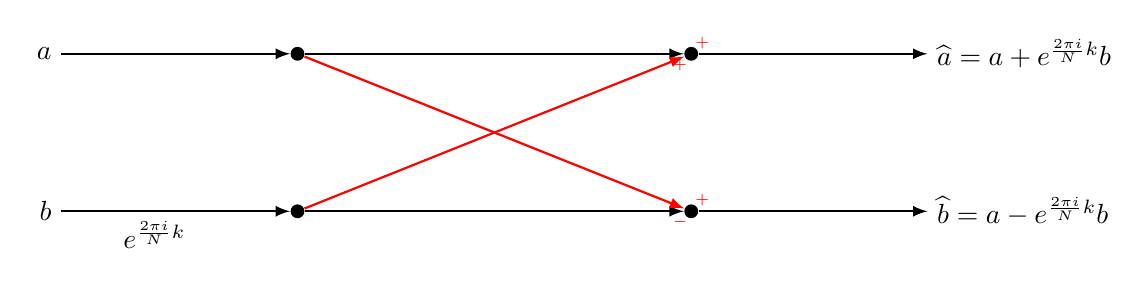
\begin{tikzpicture}[y=-1cm]

\node (A0) at (0, 0) [left]{$a$};
\node (B0) at (0, 2) [left]{$b$};

\node[circle,fill=black,minimum size=5pt,inner sep=0pt] (A1) at (3, 0) {};
\node[circle,fill=black,minimum size=5pt,inner sep=0pt] (B1) at (3, 2) {};

\draw[-latex,thick] (A0) -- (A1);
\draw[-latex,thick] (B0) -- (B1);

\node (B0) at (1.7, 2.3) [left]{$e^{\frac{2 \pi i}{N}k}$};


\node[circle,fill=black,minimum size=5pt,inner sep=0pt] (A2) at (8, 0) {};
\node[circle,fill=black,minimum size=5pt,inner sep=0pt] (B2) at (8, 2) {};

\draw[-latex,thick] (A1) -- (A2);
\draw[-latex,thick] (B1) -- (B2);

\draw[-latex,thick,red] (A1) -- (B2);
\draw[-latex,thick,red] (B1) -- (A2);

\node[red] at (A2) [shift={(315:0.2)}] {\tiny$+$};
\node[red] at (A2) [shift={(135:0.2)}] {\tiny$+$};
\node[red] at (B2) [shift={(315:0.2)}] {\tiny$+$};
\node[red] at (B2) [shift={(135:0.2)}] {\tiny$-$};

\node (A3) at (11, 0) [right]{$\widehat{a}=a + e^{\frac{2 \pi i}{N}k} b$};
\node (B3) at (11, 2) [right]{$\widehat{b}=a - e^{\frac{2 \pi i}{N}k} b$};

\draw[-latex,thick] (A2) -- (A3);
\draw[-latex,thick] (B2) -- (B3);

\end{tikzpicture}

\caption{Basic butterfly diagram in the decimation-in-time FFT algorithm}
\label{fig:butterfly_basic}
\end{figure}

The basic computation in \ref{eq:fft_butterfly} is called the \textit{butterfly} structure because the flow graph resembles a butterfly as shown in Figure \ref{fig:butterfly_basic}.
It is the basic computation performed in the radix-2 FFT. It can be seen that by this process the number of complex multiplications has been reduced from $N^2$ to $N^2/2+N/2$. We can repeat this process, the so-called 
\textit{decimation-in-time}, recursively for both $f_1[n]$ and $f_2[n]$. For $N=2^{\nu}$, this decimation can be performed $\nu$ times reducing the number of multiplications to 
$\frac{N}{2}\log_2 N$ and the number of additions to $N \log_2 N$.

For illustration, Figure \ref{fig:butterfly_fft} depicts the computation of an $N=8$-point DFT. In three stages, first 4 two-point DFTs are computed, then 2 four-point DFTS and 
lastly one 8-point DFT. These smaller DFTs are combined in a butterfly structure to form the larger DFT.

\begin{figure}

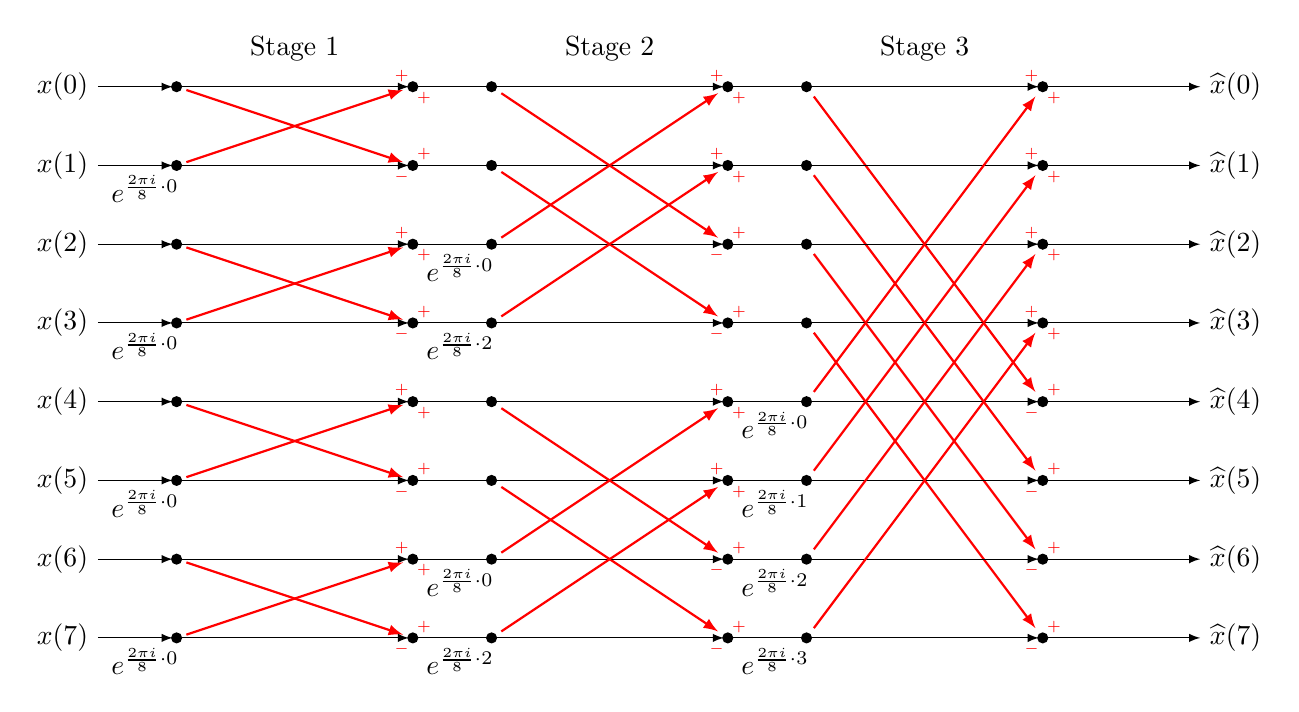
\begin{tikzpicture}[y=-1cm]

\node (t1) at (1.5, -0.2) [above]{Stage 1};
\node (t2) at (5.5, -0.2) [above]{Stage 2};
\node (t3) at (9.5, -0.2) [above]{Stage 3};


\foreach\y in {0,...,7} 
{
  \pgfmathtruncatemacro\yy{mod(abs(3.5-\y)+0.5,2)==0?\y:(\y<4?\y+3:\y-3)} % F value
  \draw[-latex] (-1,\y) node [left] {$x(\y)$} -- (-0.05,\y);
  \draw[-latex] (12,\y) -- (13,\y) node [right] {$\widehat{x}(\y)$};
  \foreach\x in {0,1,2}
  {
    \draw[-latex] (4*\x,\y) --++ (2.95,0) ;
    \draw(4*\x+3,\y) --++ (1,0);
    \foreach\z in {0,3}
      \node[circle,fill,inner sep=0.5mm] at (4*\x+\z,\y) {};
    \pgfmathtruncatemacro\i{pow(2,\x)}
    \pgfmathtruncatemacro\j{\i-2*\i*mod(div(\y,\i),2)} % delta y for the arrows
    \node (A) at (4*\x,\y)      {};
    \node (B) at (4*\x+3,\y+\j) {};
    \draw[-latex,thick,red] (A) -- (B);
    \ifnum\j < 0
      \node[red] at (B) [shift={(225:0.2)}] {\tiny$+$};
      \node[red] at (B) [shift={ (45:0.2)}] {\tiny$+$};
    \else
      \pgfmathtruncatemacro\k{mod(\y,\i)*(2-abs(\x-1))} % W exponent
      \node[red] at (B) [shift={(315:0.2)}] {\tiny$+$};
      \node[red] at (B) [shift={(135:0.2)}] {\tiny$-$};
      \node at (4*\x-0.8, \y+\j) [shift={(0.4,0.3)}] {$e^{\frac{2 \pi i}{8}\cdot \k}$};
    \fi
  }
}
\end{tikzpicture}
\caption{Visualization of a 3 stage radix-2 FFT algorithm}
\label{fig:butterfly_fft}
\end{figure}

Implementing the FFT efficiently poses further challenges that I will not cover here. In this work I will use the FFTW library, implementation and design details
can be found in \cite{FFTW.jl-2005}.

